\documentclass[aspectratio=169]{beamer}

\usetheme{Boadilla}
\usefonttheme{professionalfonts}
\setbeamertemplate{navigation symbols}{}
\setbeamertemplate{itemize items}[circle]
\setbeamertemplate{enumerate items}[default]
\setbeamertemplate{headline}{}

\usepackage[utf8]{inputenc}
\usepackage[T1]{fontenc}
\usepackage{lmodern}
\usepackage{amsmath}
\usepackage{booktabs}
\usepackage{tabularx}
\usepackage{array}
\usepackage{hyperref}
\usepackage[strings]{underscore}
\usepackage{listings}
\usepackage{tikz}
\usetikzlibrary{arrows.meta,positioning,fit,calc,shapes.geometric}
\usepackage{xcolor}

\definecolor{courseblue}{HTML}{12355B}
\definecolor{coursegold}{HTML}{C98A2E}
\definecolor{courseice}{HTML}{EEF3F8}
\definecolor{coursegreen}{HTML}{2F6B4F}
\definecolor{coursegray}{HTML}{4B5563}
\definecolor{codebg}{HTML}{F7F9FC}
\definecolor{codecomment}{HTML}{5E6C84}
\definecolor{codestring}{HTML}{0B6E4F}

\setbeamercolor{palette primary}{bg=courseblue,fg=white}
\setbeamercolor{palette secondary}{bg=coursegold,fg=white}
\setbeamercolor{palette tertiary}{bg=courseblue,fg=white}
\setbeamercolor{palette quaternary}{bg=coursegold,fg=white}
\setbeamercolor{structure}{fg=courseblue}
\setbeamercolor{frametitle}{bg=courseice,fg=courseblue}
\setbeamercolor{title}{fg=courseblue}
\setbeamercolor{block title}{bg=courseblue,fg=white}
\setbeamercolor{block body}{bg=courseice,fg=black}
\setbeamercolor{normal text}{fg=black,bg=white}
\setbeamercolor{alerted text}{fg=coursegold}

\setbeamerfont{footline}{size=\scriptsize}

\setbeamertemplate{footline}{
  \leavevmode
  \hbox{
    \begin{beamercolorbox}[wd=.33\paperwidth,ht=2.8ex,dp=1.2ex,leftskip=0.8em]{palette primary}%
      University of Trieste
    \end{beamercolorbox}%
    \begin{beamercolorbox}[wd=.49\paperwidth,ht=2.8ex,dp=1.2ex,center]{palette tertiary}%
      \coursename{} \textbar{} \coursecode
    \end{beamercolorbox}%
    \begin{beamercolorbox}[wd=.18\paperwidth,ht=2.8ex,dp=1.2ex,rightskip=0.8em plus1fil]{palette secondary}%
      \insertframenumber{} / \inserttotalframenumber
    \end{beamercolorbox}%
  }
}

\hypersetup{
  colorlinks=true,
  linkcolor=courseblue,
  urlcolor=coursegreen
}

\lstdefinestyle{coursepython}{
  language=Python,
  basicstyle=\ttfamily\footnotesize,
  keywordstyle=\color{courseblue}\bfseries,
  commentstyle=\color{codecomment}\itshape,
  stringstyle=\color{codestring},
  showstringspaces=false,
  columns=fullflexible,
  keepspaces=true,
  frame=single,
  framerule=0.6pt,
  rulecolor=\color{courseblue},
  backgroundcolor=\color{codebg},
  xleftmargin=0.4em,
  xrightmargin=0.4em,
  aboveskip=0.4em,
  belowskip=0.2em
}

\newcommand{\coursename}{Data-driven Systems Engineering}
\newcommand{\coursecode}{440MI / 305SM}
\newcommand{\coursefooter}{}

\newcommand{\learninggoals}[1]{
  \begin{block}{Learning goals}
  #1
  \end{block}
}

\newcommand{\repoactivity}[1]{
  \begin{block}{Repo activity}
  #1
  \end{block}
}

\newcommand{\readinglist}[1]{
  \begin{block}{Papers and materials}
  {\footnotesize #1}
  \end{block}
}

\newcommand{\coursecontextframe}[5]{
  \begin{frame}{Course Map and Running Cases}
  \centering
  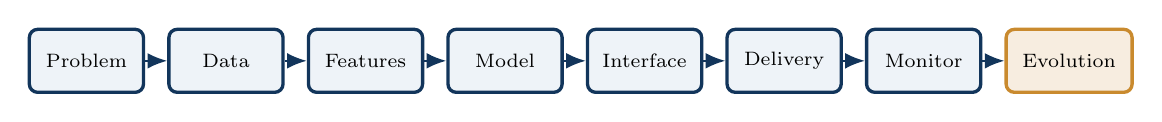
\begin{tikzpicture}[node distance=0.28cm]
  \node[flowbox, minimum width=1.45cm, minimum height=0.8cm] (problem) {\scriptsize Problem};
  \node[flowbox, minimum width=1.45cm, minimum height=0.8cm, right=of problem] (data) {\scriptsize Data};
  \node[flowbox, minimum width=1.45cm, minimum height=0.8cm, right=of data] (features) {\scriptsize Features};
  \node[flowbox, minimum width=1.45cm, minimum height=0.8cm, right=of features] (model) {\scriptsize Model};
  \node[flowbox, minimum width=1.45cm, minimum height=0.8cm, right=of model] (interface) {\scriptsize Interface};
  \node[flowbox, minimum width=1.45cm, minimum height=0.8cm, right=of interface] (delivery) {\scriptsize Delivery};
  \node[flowbox, minimum width=1.45cm, minimum height=0.8cm, right=of delivery] (monitor) {\scriptsize Monitor};
  \node[accentbox, minimum width=1.6cm, minimum height=0.8cm, right=of monitor] (evolution) {\scriptsize Evolution};
  \foreach \a/\b in {problem/data,data/features,features/model,model/interface,interface/delivery,delivery/monitor,monitor/evolution} {
    \draw[arrow] (\a) -- (\b);
  }
  \end{tikzpicture}

  \vspace{0.5em}
  \begin{block}{Today in the course}
  \textbf{Focus:} #1

  \textbf{Bridge:} #2
  \end{block}

  \begin{columns}[T]
  \column{0.48\textwidth}
  \begin{block}{Fraud case}
  {\footnotesize #3}
  \end{block}
  \column{0.48\textwidth}
  \begin{block}{Pasteurization case}
  {\footnotesize #4}
  \end{block}
  \end{columns}

  \vspace{0.3em}
  {\footnotesize \textbf{Course thread:} #5}
  \coursefooter
  \end{frame}
}

\newcommand{\classclosingframe}[4]{
  \begin{frame}{From This Class to the Next}
  \begin{block}{What stays with us}
  #1
  \end{block}

  \begin{columns}[T]
  \column{0.48\textwidth}
  \begin{block}{Project use}
  {\footnotesize #2}
  \end{block}
  \column{0.48\textwidth}
  \begin{block}{Next connection}
  {\footnotesize #3}
  \end{block}
  \end{columns}

  \vspace{0.3em}
  {\footnotesize \textbf{Course thread:} #4}
  \coursefooter
  \end{frame}
}

\tikzset{
  flowbox/.style={
    rounded corners=3pt,
    draw=courseblue,
    fill=courseice,
    very thick,
    minimum width=2.2cm,
    minimum height=0.9cm,
    align=center,
    font=\small
  },
  accentbox/.style={
    rounded corners=3pt,
    draw=coursegold,
    fill=coursegold!15,
    very thick,
    minimum width=2.2cm,
    minimum height=0.9cm,
    align=center,
    font=\small
  },
  arrow/.style={
    -{Latex[length=2.5mm,width=2mm]},
    thick,
    draw=courseblue
  }
}


\title{Class 4: Python --- Control Flow and Data Structures}
\author{\coursename}
\date{}

\begin{document}

\frame{\titlepage \coursefooter}

\begin{frame}{Agenda}
\begin{itemize}
\item Conditionals: making decisions with \texttt{if} / \texttt{elif} / \texttt{else}.
\item For loops, \texttt{enumerate}, and list comprehensions.
\item While loops and when to prefer them.
\item Dictionaries: key--value pairs beyond the list.
\item Writing your first functions with \texttt{def}.
\item Why loops eventually hand off to NumPy and Matplotlib.
\end{itemize}
\coursefooter
\end{frame}

\begin{frame}{Learning goals}
\learninggoals{
\begin{itemize}
\item Write conditional logic using comparison and boolean operators.
\item Iterate over a list with a \texttt{for} loop, with and without \texttt{enumerate}.
\item Build a list with a comprehension, with and without a filter condition.
\item Create, read, and iterate over a dictionary.
\item Define a small function with \texttt{def} and call it correctly.
\end{itemize}
}
\coursefooter
\end{frame}

\coursecontextframe
{Control flow and the two data structures --- lists and dictionaries --- that carry most Python logic.}
{Last class gave us values; this class gives those values a way to branch, repeat, and be looked up by name.}
{The fraud dashboard loops over 28 behavioral features to build one input vector, and a hyperparameter search is itself just a dictionary of lists.}
{The pasteurization simulator loops over sensor batches and branches on process state --- ``heating,'' ``holding,'' ``cooling'' --- using exactly this vocabulary.}
{Every later pipeline is a composition of loops, conditionals, and lookups; today we name each piece explicitly.}

\begin{frame}{Conditionals}
\begin{itemize}
\item \texttt{if}, \texttt{elif}, and \texttt{else} branch execution based on a boolean expression.
\item Comparisons: \texttt{==}, \texttt{!=}, \texttt{<}, \texttt{<=}, \texttt{>}, \texttt{>=}.
\item Python uses indentation, not braces, to mark which statements belong to a branch.
\item A colon \texttt{:} always introduces the indented block that follows.
\end{itemize}
\coursefooter
\end{frame}

\begin{frame}[fragile]{Conditionals in practice}
\begin{lstlisting}[style=coursepython]
if prediction == 1:
    st.error(f"High risk of fraud: {probability:.2%}")
else:
    st.success(f"Transaction appears legitimate: {probability:.2%}")
\end{lstlisting}
\begin{itemize}
\item This is the decision at the heart of `App_Credit_Card.py`: one comparison, two branches.
\item Note the \texttt{\#} comment convention is skipped here because the branch itself is self-explanatory --- a first taste of the readability habits we formalize in Class 7.
\end{itemize}
\coursefooter
\end{frame}

\begin{frame}[fragile]{For loops}
\begin{lstlisting}[style=coursepython]
for i in range(1, 29):
    col = cols[(i - 1) % 3]
    user_inputs.append(
        col.slider(f"Feature V{i}", -5.0, 5.0, 0.0, step=0.1)
    )
\end{lstlisting}
\begin{itemize}
\item \texttt{for} iterates over a sequence --- here, \texttt{range(1, 29)} produces the numbers 1 through 28.
\item This is the real loop in `App_Credit_Card.py` that builds the 28 feature sliders V1 through V28.
\item The list \texttt{user\_inputs} from last class is exactly what this loop fills in, one \texttt{.append()} at a time.
\end{itemize}
\coursefooter
\end{frame}

\begin{frame}{\texttt{enumerate} and list comprehensions}
\begin{itemize}
\item \texttt{enumerate(sequence)} gives both the index and the value in one loop, avoiding manual counters.
\item A list comprehension builds a list in one line: \texttt{[expr for item in sequence]}.
\item Comprehensions can filter: \texttt{[expr for item in sequence if condition]}.
\item Comprehensions do not replace every loop --- they shine when the loop body is a single transformation.
\end{itemize}
\coursefooter
\end{frame}

\begin{frame}[fragile]{Comprehension example}
\begin{lstlisting}[style=coursepython]
feature_names = [f"V{i}" for i in range(1, 29)]
high_risk_features = [f for f in feature_names if f != "V1"]
\end{lstlisting}
\begin{itemize}
\item The first line generates the same 28 feature labels the sliders use, without a manual loop.
\item The second line adds a filter condition --- the comprehension form of an \texttt{if} inside a \texttt{for}.
\end{itemize}
\coursefooter
\end{frame}

\begin{frame}{While loops}
\begin{itemize}
\item \texttt{while condition:} repeats a block as long as the condition stays true.
\item Useful when the number of iterations is not known in advance, unlike a \texttt{for} loop over a fixed sequence.
\item Streaming and monitoring code --- reading sensor batches until a stream ends --- is a natural \texttt{while} use case, previewed later in the pasteurization service.
\item A missing update to the loop variable is the classic beginner bug: an infinite loop.
\end{itemize}
\coursefooter
\end{frame}

\begin{frame}[fragile]{Dictionaries}
\begin{lstlisting}[style=coursepython]
param_grid = {
    'n_estimators': [50, 100, 200],
    'max_depth': [3, 5, 8, None],
    'min_samples_split': [2, 4, 6]
}

for key, value in param_grid.items():
    print(key, value)
\end{lstlisting}
\begin{itemize}
\item A dictionary stores key--value pairs, similar to a map: look up a value by its key instead of by position.
\item This exact dictionary comes from `notebooks/Class6_Model_Training_.ipynb`; note the values are themselves lists.
\item \texttt{.items()} is the built-in way to iterate over both keys and values together.
\end{itemize}
\coursefooter
\end{frame}

\begin{frame}{Writing your first functions}
\begin{itemize}
\item Functions are defined with \texttt{def name(parameters):} followed by an indented body.
\item \texttt{return} sends a value back to the caller; without it, a function returns \texttt{None}.
\item Wrapping repeated logic in a function is the first step away from copy-pasted code.
\item Class 7 comes back to functions in depth --- naming, structure, and good practice; today is only the syntax.
\end{itemize}
\coursefooter
\end{frame}

\begin{frame}[fragile]{A first function}
\begin{lstlisting}[style=coursepython]
def summarize(values):
    return min(values), max(values), sum(values) / len(values)

low, high, avg = summarize(user_inputs)
\end{lstlisting}
\begin{itemize}
\item One function, three values returned as a tuple, unpacked directly into three variables.
\item This is close to the practice exercise waiting in Class 5: mean, standard deviation, minimum, and maximum of a list, behind a Streamlit front end.
\end{itemize}
\coursefooter
\end{frame}

\begin{frame}{Why loops eventually hand off to NumPy}
\begin{itemize}
\item A Python \texttt{for} loop over thousands of sensor readings or transaction rows is correct but slow.
\item NumPy performs the same arithmetic on whole arrays at once, in compiled code under the hood.
\item Matplotlib then turns those arrays into the plots we will build starting in Class 6.
\item The mental model does not change: control flow, values, containers --- only the execution engine gets faster.
\end{itemize}
\coursefooter
\end{frame}

\begin{frame}{How the repo already uses today's building blocks}
\repoactivity{
\begin{itemize}
\item `streamlit/pages/App_Credit_Card.py` uses exactly the \texttt{if}/\texttt{else} and \texttt{for} patterns shown today to build its inputs and its verdict.
\item `notebooks/Class6_Model_Training_.ipynb` defines \texttt{param\_grid} as a dictionary of lists before any model is trained.
\item Trace one loop and one dictionary in either file and describe, in your own words, what each iteration or lookup does.
\end{itemize}
}
\coursefooter
\end{frame}

\begin{frame}{Discussion prompt}
\begin{block}{Question}
The slider loop in `App_Credit_Card.py` runs exactly 28 times, always. Where in this course might a loop instead need to run an unknown number of times, and which loop would you reach for?
\end{block}
\begin{itemize}
\item Connects \texttt{for} versus \texttt{while} to a concrete forthcoming case: streaming sensor batches.
\end{itemize}
\coursefooter
\end{frame}

\begin{frame}{Papers and materials}
\readinglist{
\href{https://pandas.pydata.org/docs/}{pandas documentation};\
\href{https://scikit-learn.org/stable/}{scikit-learn documentation};\
Chip Huyen, \textit{Designing Machine Learning Systems}.
}
\coursefooter
\end{frame}

\classclosingframe
{\begin{itemize}
\item Conditionals and loops turn static values into behavior; dictionaries add lookup by name instead of position.
\item Functions package repeated logic under one name, ready for reuse.
\item The same handful of constructs already runs the fraud dashboard and the model-training notebook.
\end{itemize}}
{Before your project grows past a few lines, check whether a repeated block should already be a loop, a comprehension, or a function.}
{Class 5 puts these constructs to work in a hands-on Streamlit practice session, building a small interactive app end to end.}
{Vocabulary becomes skill only once you use it to build something that runs.}

\end{document}
